\section{Data storage and management system}

%%%%%%%%%%%%%%%%%%%%%%%%
\subsection{The \pdsp data characteristics}
Characteristics of the \pdsp data are in large part defined by a few fundamental
properties of the \pdsp Liquid Argon TPC:
\begin{itemize}
\item the high spatial granularity of the detector (e.g., the pitch of the wires, etc), and the resulting high channel count;
\item high digitization frequency (which is essential to ensure a precise position measurement along the drift direction); and
\item relatively slow drift velocity of electrons in LAr, which requires a substantial readout window (of the order of milliseconds)  to collect
all of the ionization in the LAr volume stemming from the event of interest and overlapping cosmic rays.
\end{itemize}

%\noindent 
Triggered readouts of the detector, denoted ``events'' here, 
thus contain a significant amount of raw data, impacting the bandwidth and
storage requirements.   The run plan, which determines the total number of required events, 
helps define the design requirements for the data storage and management system.

The \textit{``\pdsp Data Scenarios''} spreadsheet\,\cite{data_spreadsheet}  %(DUNE DocDB 1086)
describes a few possible running conditions. It includes estimates for their
resulting data volumes and rates, and interpretations of these estimates in terms of
network and disk bandwidth. The set of conditions labeled as ``Central'' represents the most likely scenario
and is correlated with the current run plan (see Section~\ref{sec:runplan}).
% maxim: fixed
% \fixme{Should briefly describe what the 3 running conditions are}
 It also includes estimates for non-beam
data in order to constrain the contributions of cosmic rays to the beam-on data.  Some highlights
of these estimates for the ``most likely'' scenario
can be found in Table~\ref{tab:goldi}.

Based on the estimated event-readout size quoted in Table~\ref{tab:goldi}  the anticipated raw data volume to be taken during the planned SPS run
amounts to about 3\,PB.



%%%%%%%%%%%%%%%%%%%%%%%%
\subsection{Raw data flow}
\label{sec:raw_concept}

\begin{figure}[tbh]
\centering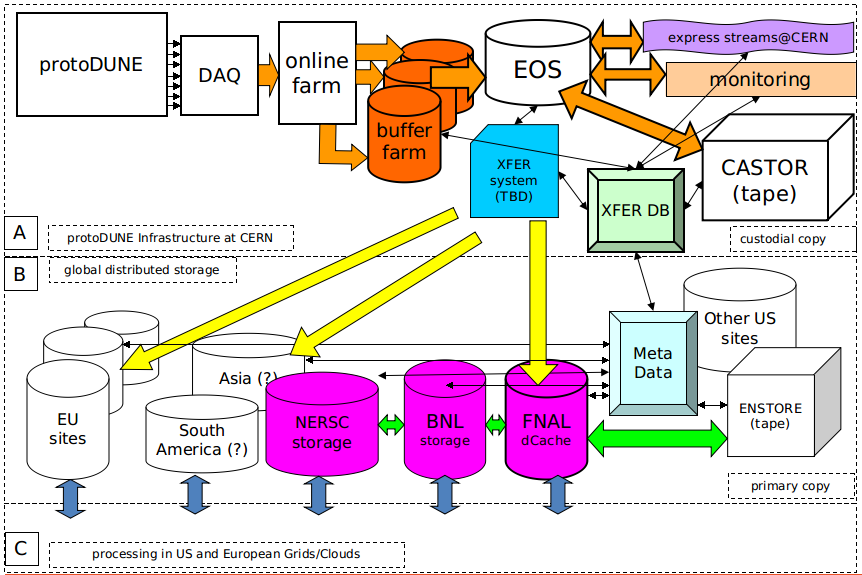
\includegraphics[width=\linewidth]{protoDUNE_raw_data_concept.png}
\caption{\label{fig:raw_concept}Conceptual diagram of the flow of raw data in \pdsp}
\end{figure}


A conceptual diagram of the raw data flow in \pdsp is presented in Figure~\ref{fig:raw_concept}. It shows the general logic
of the data flow and does not rely on assumptions of specific technical implementations. 
It also reflects the central role of CERN EOS in the \pdsp raw data management scheme which is motivated by the experience
and architecture of the LHC experiments.

EOS serves as the staging area from which the data are committed to CASTOR
and from which data are transmitted to a number of endpoints including principal data centers such as FNAL and others.
It is also used to provide input to QA and other express processing streams at CERN (Section~\ref{sec:prompt_processing}).

